%%%%%%%%%%%%%%%%%%%%%%%%%%%%%%%%%%%%%%%%%
% FRI Data Science_report LaTeX Template
% Version 1.0 (28/1/2020)
% 
% Jure Demšar (jure.demsar@fri.uni-lj.si)
%
% Based on MicromouseSymp article template by:
% Mathias Legrand (legrand.mathias@gmail.com) 
% With extensive modifications by:
% Antonio Valente (antonio.luis.valente@gmail.com)
%
% License:
% CC BY-NC-SA 3.0 (http://creativecommons.org/licenses/by-nc-sa/3.0/)
%
%%%%%%%%%%%%%%%%%%%%%%%%%%%%%%%%%%%%%%%%%


%----------------------------------------------------------------------------------------
%	PACKAGES AND OTHER DOCUMENT CONFIGURATIONS
%----------------------------------------------------------------------------------------
\documentclass[fleqn,moreauthors,10pt]{ds_report}
\usepackage[english]{babel}
\usepackage{tabularx}

\graphicspath{{fig/}}




%----------------------------------------------------------------------------------------
%	ARTICLE INFORMATION
%----------------------------------------------------------------------------------------

% Header
\JournalInfo{FRI Natural language processing course 2025}

% Interim or final report
\Archive{Project report} 
%\Archive{Final report} 

% Article title
\PaperTitle{Automatic generation of Slovenian traffic news for RTV Slovenija} 

% Authors (student competitors) and their info
\Authors{Janez Kuhar, Veljko Dudić, and Marko Rozman}

% Advisors
\affiliation{\textit{Advisors: Slavko Žitnik}}

% Keywords
\Keywords{}
\newcommand{\keywordname}{Keywords}


%----------------------------------------------------------------------------------------
%	ABSTRACT
%----------------------------------------------------------------------------------------

\Abstract{
In this report we present the related works, initial ideas and proposed dataset for our project.
}

%----------------------------------------------------------------------------------------

\begin{document}

% Makes all text pages the same height
\flushbottom 

% Print the title and abstract box
\maketitle 

% Removes page numbering from the first page
\thispagestyle{empty} 

%----------------------------------------------------------------------------------------
%	ARTICLE CONTENTS
%----------------------------------------------------------------------------------------

\section*{Introduction}
The project focuses on replacing the manual production of traffic reports with an automated system. Traffic data provided in tabular form and traffic data from the promet.si website is used to generate traffic reports according to provided specifications.

\subsection*{Motivation}

\textbf{Timely Information.} Reliable traffic updates are critical for public safety and efficient transportation management.\\
\textbf{Manual Process Limitations.} Currently, students manually verify and type these reports every 30 minutes, leading to potential delays and inaccuracies.\\
\textbf{Automated Solution.} By utilizing LLMs and advanced prompt engineering (inspired by works on news headline generation), we aim to generate clear, concise, and contextually accurate traffic news.

\section{Related Work}

Li et al. \cite{liHGNewsNewsHeadline2021} proposed a decoder-only model for headline generation,
incorporating multihead attention, sentiment features, and part-of-speech information. Its focus
on generating succinct news headlines while accurately handling out-of-vocabulary
terms (such as specific road names) can be directly applicable to our task.

In a more recent work on the topic of text summarization \cite{houAlgorithmAutomaticAbstract2024}, a ChatGPT-based
algorithm for summarizing Russian texts was proposed. The suggested approach combined preprocessing (e.g., word segmentation,
stop word removal) with BERT for contextual understanding and a pointer mechanism for out-of-vocabulary
words.

Sha et al. \cite{sha2018order} proposed an order-planning mechanism for text generation from tabular data, combining
link-based attention with traditional content-based attention to model the sequence of information. Their approach
was further enhanced by a copy mechanism to handle rare words, improving the model's ability to generate accurate
and coherent summaries from structured data.

\section{Initial ideas}
\begin{itemize}
    \item Initial Prompt Engineering: Experiments will start by generating news texts directly from the structured traffic data using prompts.
    
    \item Selection of important data. Our observations show that the final news report is mostly made from only few important data points from the Excel file. We intend to filter the data to remove duplicate enteries and automaticly select the important data points relavant for our traffic news generation.
    
    \item Enhanced Generation through Fine-Tuning: The project will then incorporate parameter-efficient fine-tuning (e.g., LoRA) and retrieval techniques to further refine the generated content, ensuring correct road naming and event descriptions.
    
    \item Evaluation: A robust evaluation framework will be established using both automatic metrics (such as ROUGE, precision, recall, and F1) and human judgment to verify that the generated texts meet RTV Slovenija's standards.

    \item Pointer Mechanisms: Integrate pointer mechanisms to ensure that domain-specific terminology (e.g., road names and traffic event descriptors) is accurately reproduced, minimizing the risk of omitting critical details.

    \item Advanced Preprocessing: Apply rigorous preprocessing techniques—such as tokenization, normalization, and filtering—to both the traffic data and guideline documents. This will help standardize the input and ensure adherence to established formats.

    \item N-gram Language Features: Incorporate n-gram features to improve language fluency and ensure that generated sentences are coherent and stylistically consistent with existing RTV Slovenija news.

    \end{itemize}

\section{Methods}

\subsection*{Project dataset}

The primary dataset was provided to us by the TA. It consists of three important sets of files:

\begin{enumerate}
    \item \textbf{A structured Excel }file containing historical traffic report information from \textit{promet.si}.
    \item \textbf{Word documents} with lexical notes and the prescribed structure of a traffic report.
    \item \textbf{Ground truth data} in Rich Text Format (RTF) files, providing text in a ready-to-use format for radio hosts.
\end{enumerate}


\subsection*{Data preprocessing}
The pipeline first loads the RTF files and extracts dates and times embedded in their content. For each rtf file it then selects 10 previous rows. It extracts relavent columns (namely A1, B1, ContentPomembnoSLO, ContentNesreceSLO, ContentZastojiSLO, ContentVremeSLO, ContentOvireSLO, ContentDeloNaCestiSLO, ContentOpozorilaSLO, ContentMednarodneInformacijeSLO, and ContentSplosnoSLO). From each cell we extract headings and inforamtion snippets. Each snippet is then encoded using SloBERTa \cite{SloBERTa} to obtain a vector representation. We then deduplicate the snippets based on their vector representation, ensuring that only unique and relevant information is retained. Finally, we merge the headings and snippets.

We tried three different treasholds for the cosine similarity between the vectors, which resulted in different number of snippets being retained. The thresholds were set to 0.90, 0.95 and 0.99, in \ref{fig:preprocessing} we see that the higher the threshold shorter the text. After manually inspecting the results, we found that the threshold of 0.95 provided a good balance between retaining relevant information and avoiding redundancy.

\begin{figure}[h]
    \centering
    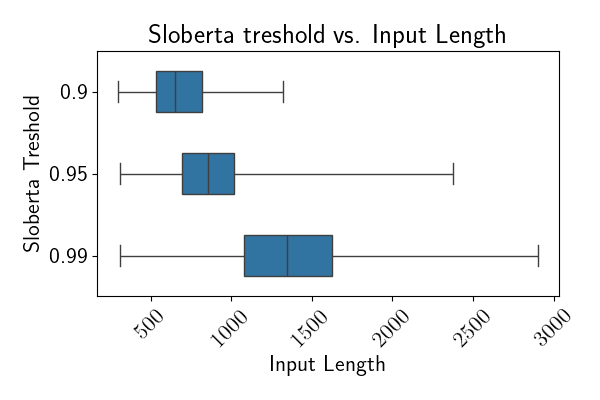
\includegraphics[width=0.8\linewidth]{fig/treshold_vs_len.png}
    \caption{Comparison of the SloBERTa treshold and text length. After manually inspecting the results, we found that the threshold of 0.95 provided a good balance between retaining relevant information and avoiding redundancy.}
    \label{fig:preprocessing}
\end{figure}



\subsection*{Prompt Engineering}

After preprocessing the tabular data, we employed a simple prompt engineering approach to generate the traffic news.
We started with a \textit{few-shot} prompting \cite{promptingguide_fewshot} technique, where we provided the model
with a few examples of preprocessed data and corresponding traffic news reports. This approach provides the model
with contextual examples, helping it mimic the structure and tone of the target traffic news format.

\subsection*{Fine-tuning}

As an extra step, we decided to fine-tune \textit{cjvt/GaMS-9B-Instruct} on our input/ground truth pairs. Since the model has 9 billion parameters and demands substantial GPU memory, we employed QLoRA to enable efficient fine-tuning for the news generation task. This approach allowed us to update only a small number of low-rank adapter weights while keeping the quantized base model frozen. Training prompts were structured as alternating user and model turns using special tokens to clearly mark role boundaries, as shown below:

\begin{verbatim}
<start_of_turn>user
...pre-processed input data...
<end_of_turn>
<start_of_turn>model
...ground truth traffic news report...
<end_of_turn>
\end{verbatim}

\subsection*{Evaluation metrics}

The evaluation focuses on the BLEU score as a measure of translation quality, with the possibility of adding other metrics in the future.

\noindent \textbf{BLEU Score:} The BLEU (Bilingual Evaluation Understudy) score is a popular metric for evaluating the quality of machine-generated text, particularly for tasks like text summarization or machine translation. It is based on precision, specifically n-gram precision, where a higher BLEU score indicates that the machine-generated text closely matches the ground truth.

The BLEU score ranges from 0 to 1, where a higher value suggests better quality. However, BLEU has limitations, especially when dealing with languages that have more varied sentence structures or when evaluating more creative text generation tasks like traffic report creation. For example, it does not account for semantic meaning and may penalize diverse word choices or paraphrasing that is still correct. Additionally, BLEU heavily relies on n-gram matching, which may penalize acceptable lexical variations. For example, if the model uses different phrasing that still conveys the same meaning, it may receive a lower BLEU score, which does not necessarily reflect a poor-quality output.


\section{Results and Evaluation}

\subsection*{Computational Resources}

Inference and training for all experiments was conducted on the ARNE HPC cluster. The cluster is equipped with NVIDIA's H100 80GB and V100 32GB GPUs, enabling efficient handling of LLMs.

\subsection*{Quantitative Results}

\vspace{1em} % adds vertical space before
\noindent \textbf{V1}
\vspace{0.5em} % adds vertical space after

For each experimental setup, we ran 32 trials to ensure statistical reliability. During each trial, a randomly sampled
set of input-output pairs was used, and the performance score was calculated for each pair.


The baseline results for few-shot prompting with GaMS-9B-Instruct \cite{huggingface2025gams9b} are listed in Table~\ref{tab:bleu-results}. We experimented with different configurations by varying the number of shots (input/output pairs) and the number of rows merged from the Excel file into a single input.
\begin{table}[h!]
    \centering
    \caption{Average BLEU scores for different few-shot prompting setups using GaMS-9B-Instruct. Each configuration was evaluated over 32 trials. \textbf{Rows}: The number of Excel rows merged into a single input. \textbf{Shots}: The number of input/output pairs presented to the model for few-shot prompting.}
    \label{tab:bleu-results}
    \small
    \begin{tabular}{@{}cccc@{}}
    \toprule
    \textbf{Rows} & \textbf{Shots} & \textbf{Trials} & \textbf{BLEU} \\
    \midrule
    1 & 8 & 32 & \textbf{0.1942} \\
    3 & 2 & 32 & \textbf{0.1576} \\
    \bottomrule
    \end{tabular}
\end{table}

As expected, increasing the number of shots provided the model with more context, which typically improves its performance. However, increasing the number of shots also resulted in higher memory consumption, so we had to find a balance that remained within our system's limits.

Interestingly, the average BLEU score decreased when we merged several Excel rows into the input. While we expected more data to improve the model's performance, the increase in data duplication led us to reduce the number of shots. With only 2 examples presented to the model, the model lacked sufficient context to recover all the relevant details from the ground truth, which likely led to missing parts in the generated reports.

\vspace{1em} % adds vertical space before
\noindent \textbf{V2}
\vspace{0.5em} % adds vertical space after

First, we fine-tuned \textit{cjvt/GaMS-9B-Instruct}. We loaded the base model weights in 4-bit (NF4) precision with
double quantization. LoRA adapters of rank $16$ ($\alpha = 32$, dropout $=0.1$) were applied to all query/value
projection layers, with no bias terms and a causal-LM objective.
Training used a JSON file of Input-GroundTruth pairs, each formatted as described in the Methods section, and
truncated to $2048$ tokens (including EOS), with $80\%$ used for training and $20\%$ held out for evaluation.
Optimization employed an AdamW-style optimizer with peak learning rate $0.0002$, linear warmup over $150$ steps
(3\% of total $5000$ steps), and gradient clipping at $0.3$. Effective batch size was $1$ (no accumulation), and
mixed precision (FP16) was used.

Next we compared inference on finetuned model with the baseline \textit{cjvt/GaMS-9B-Instruct}. The results are
shown in Figure~\ref{fig:inf_res}.

\begin{figure}[ht]
    \centering
    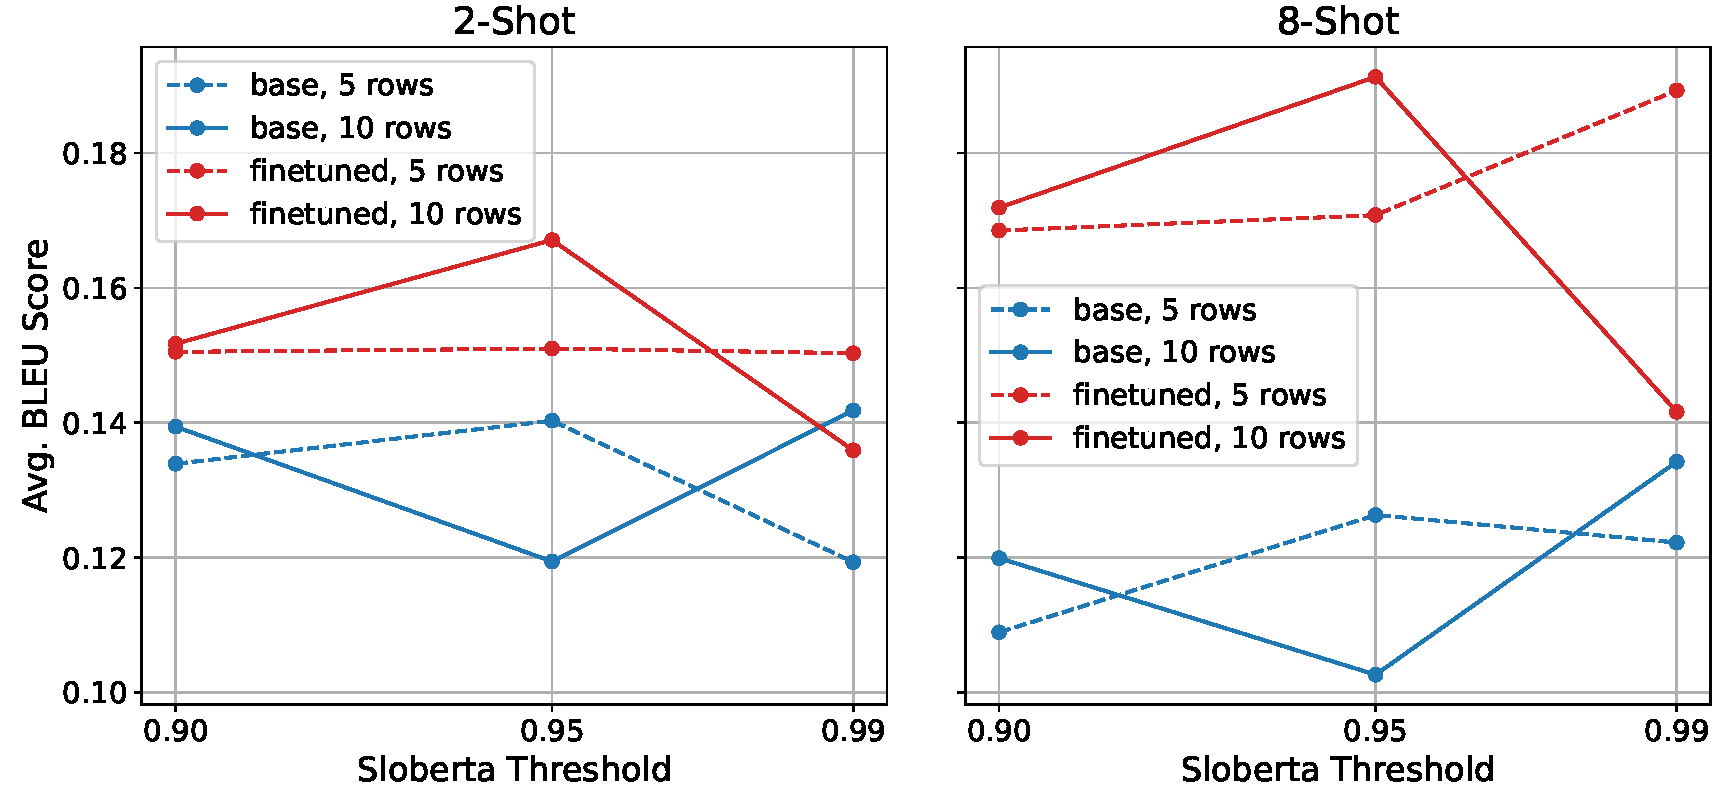
\includegraphics[width=\columnwidth]{fig/infer_res.pdf}
    \caption{Inference results comparing fine-tuned and baseline models.
    X-axis: Sloberta cosine similarity thresholds (lower = shorter input).
    Red: fine-tuned model, Blue: baseline.
    Left: 2-shot, Right: 8-shot prompting.
    Fine-tuned model shows higher BLEU scores.}
    \label{fig:inf_res}
\end{figure}

% ---------- 4.2 Qualitative Example / Error Analysis ----------
\subsection{Qualitative Example / Error Analysis}
\label{subsec:qualitative}

\vspace{1em} % adds vertical space before
\noindent \textbf{V1}
\vspace{0.5em} % adds vertical space after

To complement the quantitative BLEU scores reported in Table~\ref{tab:bleu-results}, we asked the GPT\mbox{-}o3 assistant to act as an external evaluator: it was shown one randomly selected test case from the same evaluation set and requested to assign an adequacy score on the 1–10 scale described earlier.


\begin{table}[ht]
\centering
\footnotesize                    % text a bit smaller so it wraps nicely
\renewcommand{\arraystretch}{1.15}
\setlength{\tabcolsep}{4pt}
\begin{tabularx}{\linewidth}{@{}X@{}}
\toprule
\textbf{Ground-truth bulletin} \\  % <-- row 1 heading
\midrule
\textit{Podatki o prometu. Zaradi del so zastoji na regionalni cesti Vrhnika–Ljubljana pri avtocestnem priključku Brezovica v obe smeri. Na primorski avtocesti proti Kopru je zaradi razlitega goriva vozišče spolzko med Vrhniko in Logatcem. Na vipavski hitri cesti je zaradi pokvarjenega tovornjaka med predorom Podnanos in priključkom Vipava še vedno zaprt vozni pas proti Novi Gorici. Na mejnem prehodu Obrežje vozniki tovornih vozil na vstop v državo čakajo več kot 2 uri.} \\[0.8em] % small vertical gap
\midrule

\textbf{Model-generated bulletin} \\  % <-- row 2 heading
\midrule
\textit{Podatki o prometu. Na ljubljanski obvoznici je zastoj proti Primorski, ki sega do razcepa Kozarje. Čas potovanja se tam podaljša za približno četrt ure. Na cesti Maribor – Hoče je zastoj dolg 2 kilometra. Na regionalni cesti Vrhnika – Brezovica – Ljubljana je zastoj pred delovno zaporo pri Brezovici proti Podpeči. Na cesti Podpeč – Brezovica je zastoj od Podpeči proti Brezovici. Priporočamo obvoz po avtocesti med Vrhniko in Ljubljano, vendar le za vozila opremljena z vinjeto ali napravo DarsGo. Na dolenjski avtocesti je med predoroma Mali vrh in Debeli hrib oviran promet zaradi okvare vozila. Na mejnem prehodu Obrežje vozniki tovornih vozil na vstop v državo čakajo do 2 uri.} \\
\bottomrule
\end{tabularx}
\caption{Illustrative example of expected versus generated traffic bulletin used in the OpenAI o3 adequacy evaluation.}
\label{tab:qualitative}
\end{table}

\paragraph{o3 adequacy score.}  
Using the 1–10 scale described in our annotation guidelines, this example received an \textbf{adequacy score of 4}.  The score reflects the following observations:

\begin{itemize}
  \item \textbf{Coverage:} Only one of the four critical events in the ground truth is reproduced; two are omitted entirely (slick lane Vrhnika–Logatec, lane closure Podnanos–Vipava) and one is partially correct (queues Vrhnika–Brezovica but only one direction).
  \item \textbf{Hallucinations:} Five incidents not present in the ground-truth bulletin are introduced (e.g. Ljubljana ring, Maribor–Hoče, Podpeč queues).
  \item \textbf{Detail accuracy:} Waiting time at Obrežje is understated (“do 2 uri” vs.\ “več kot 2 uri”), softening the severity.
\end{itemize}

\paragraph{Take-aways.}  
This qualitative evidence clarifies why the BLEU score ($\approx$ 0.19) remains modest despite grammatical fluency: the model tends to \emph{omit} salient facts and \emph{invent} unrelated incidents, both of which automatic n-gram metrics penalise weakly.  

% --------------------------------------------------------------

%----------------------------------------------------------------------------------------
%	REFERENCE LIST
%----------------------------------------------------------------------------------------
\bibliographystyle{unsrt}
\bibliography{report}


\end{document}
